\chapter{OpenArmor Agent-Server Testing}

\section{Introduction}
This chapter outlines the testing procedures for the OpenArmor agent-server communication. It provides a structured approach to verify the functionality, security, and performance of the interaction between OpenArmor agents and the central server infrastructure.

\begin{figure}[h]
    \centering
    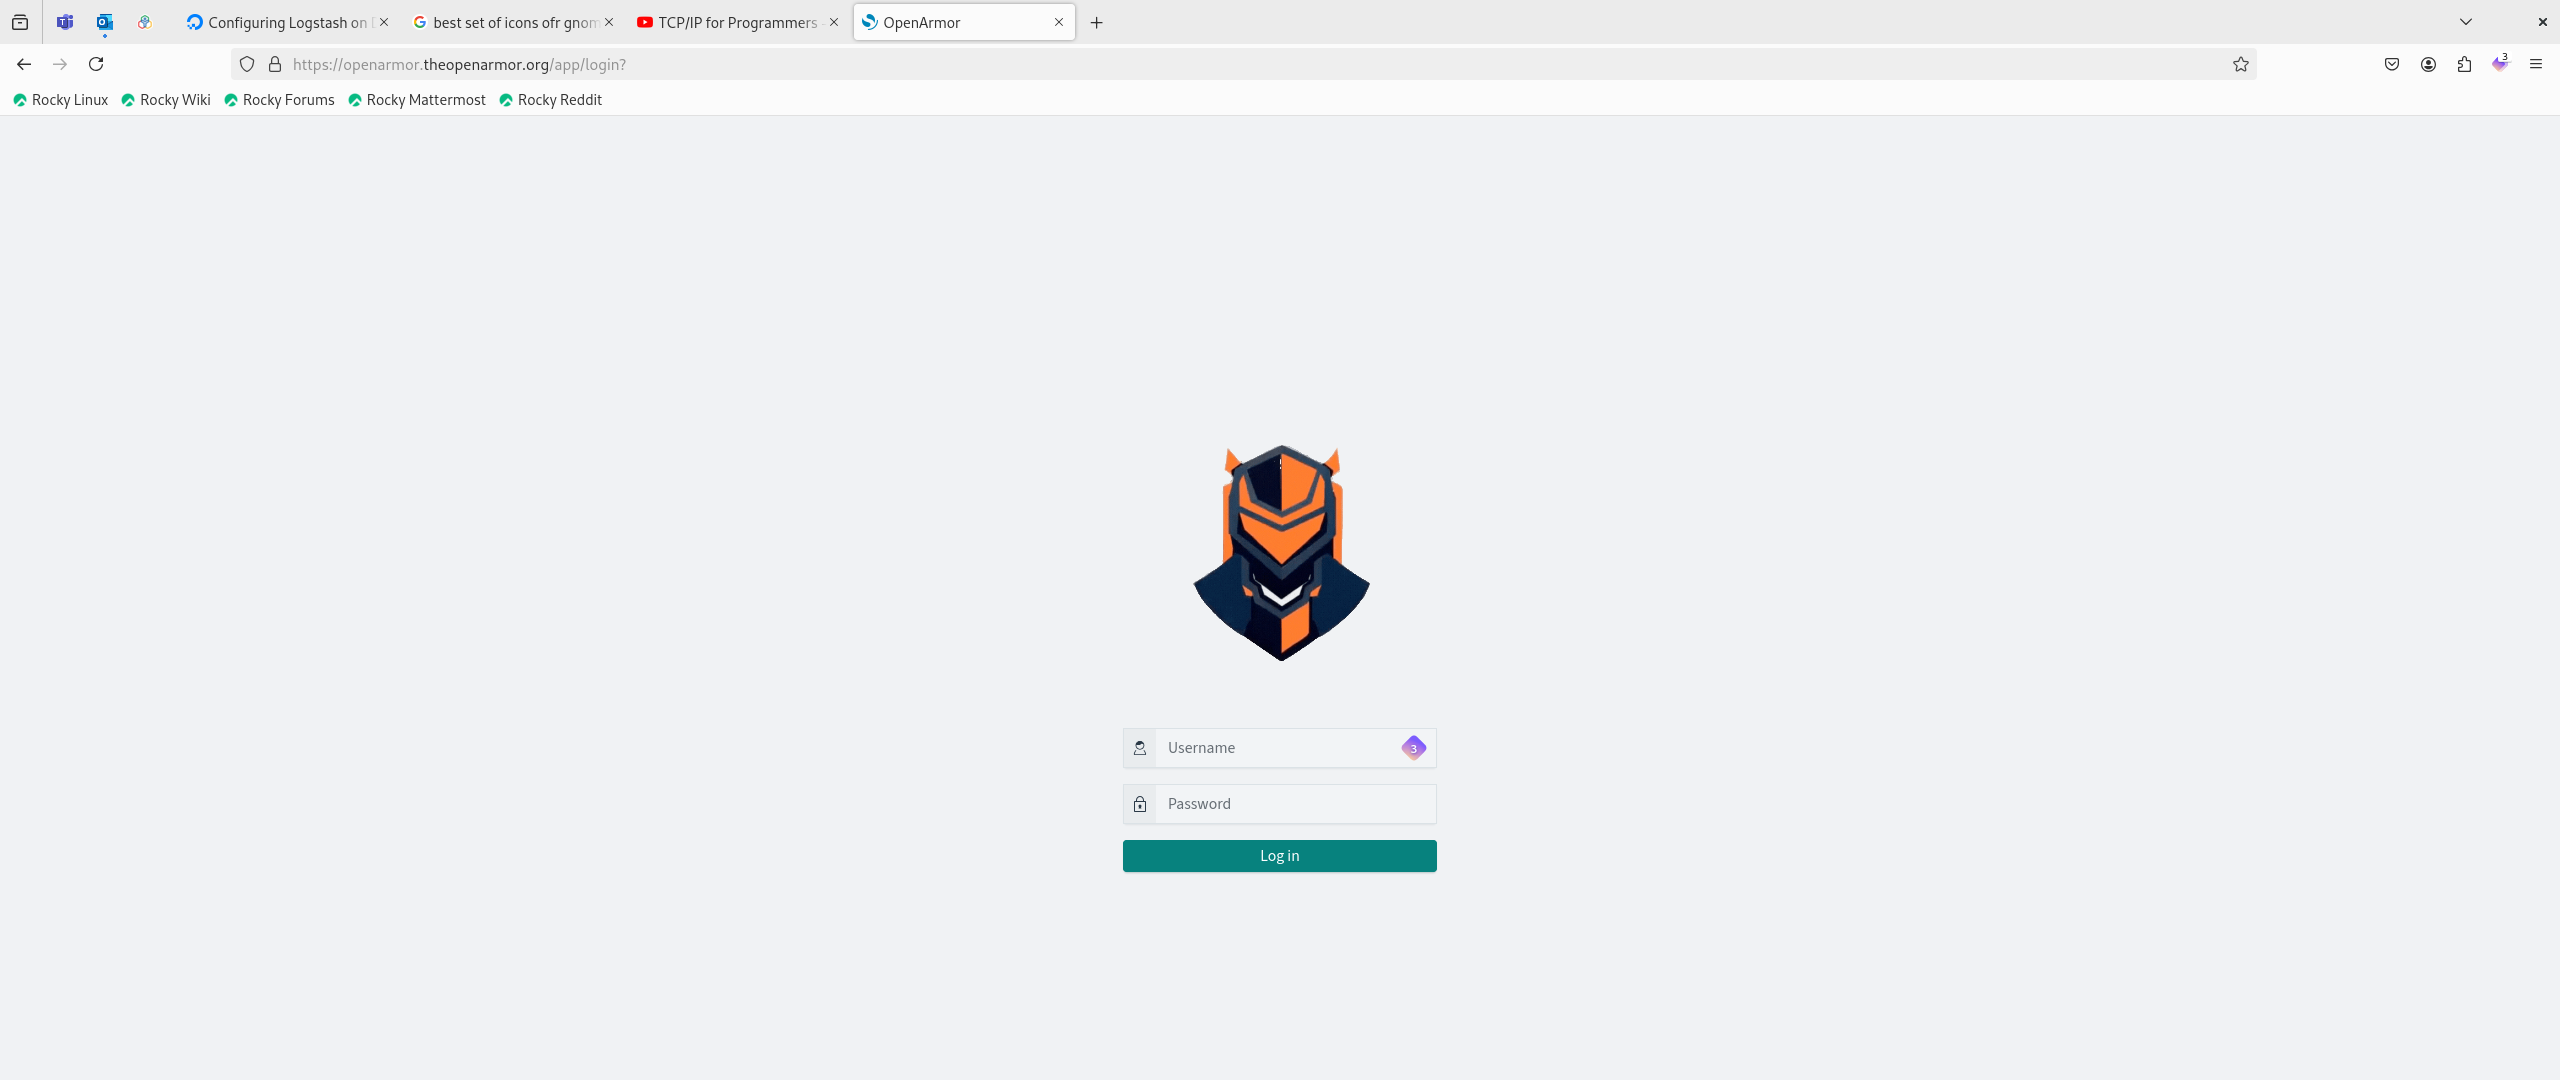
\includegraphics[width=0.8\textwidth]{openarmor-agent/1.png}
    \caption{OpenArmor Agent-Server Overview}
    \label{fig:agent-server-overview}
\end{figure}

\section{Test Environment Setup}
\subsection{Agent Setup}
\begin{enumerate}
    \item Install OpenArmor agent on test endpoints (Windows, Linux, macOS).
    \item Configure agent with test server details.
    \item Ensure all dependencies (osquery, ClamAV, Sysmon) are installed and configured.
\end{enumerate}

\begin{figure}[h]
    \centering
    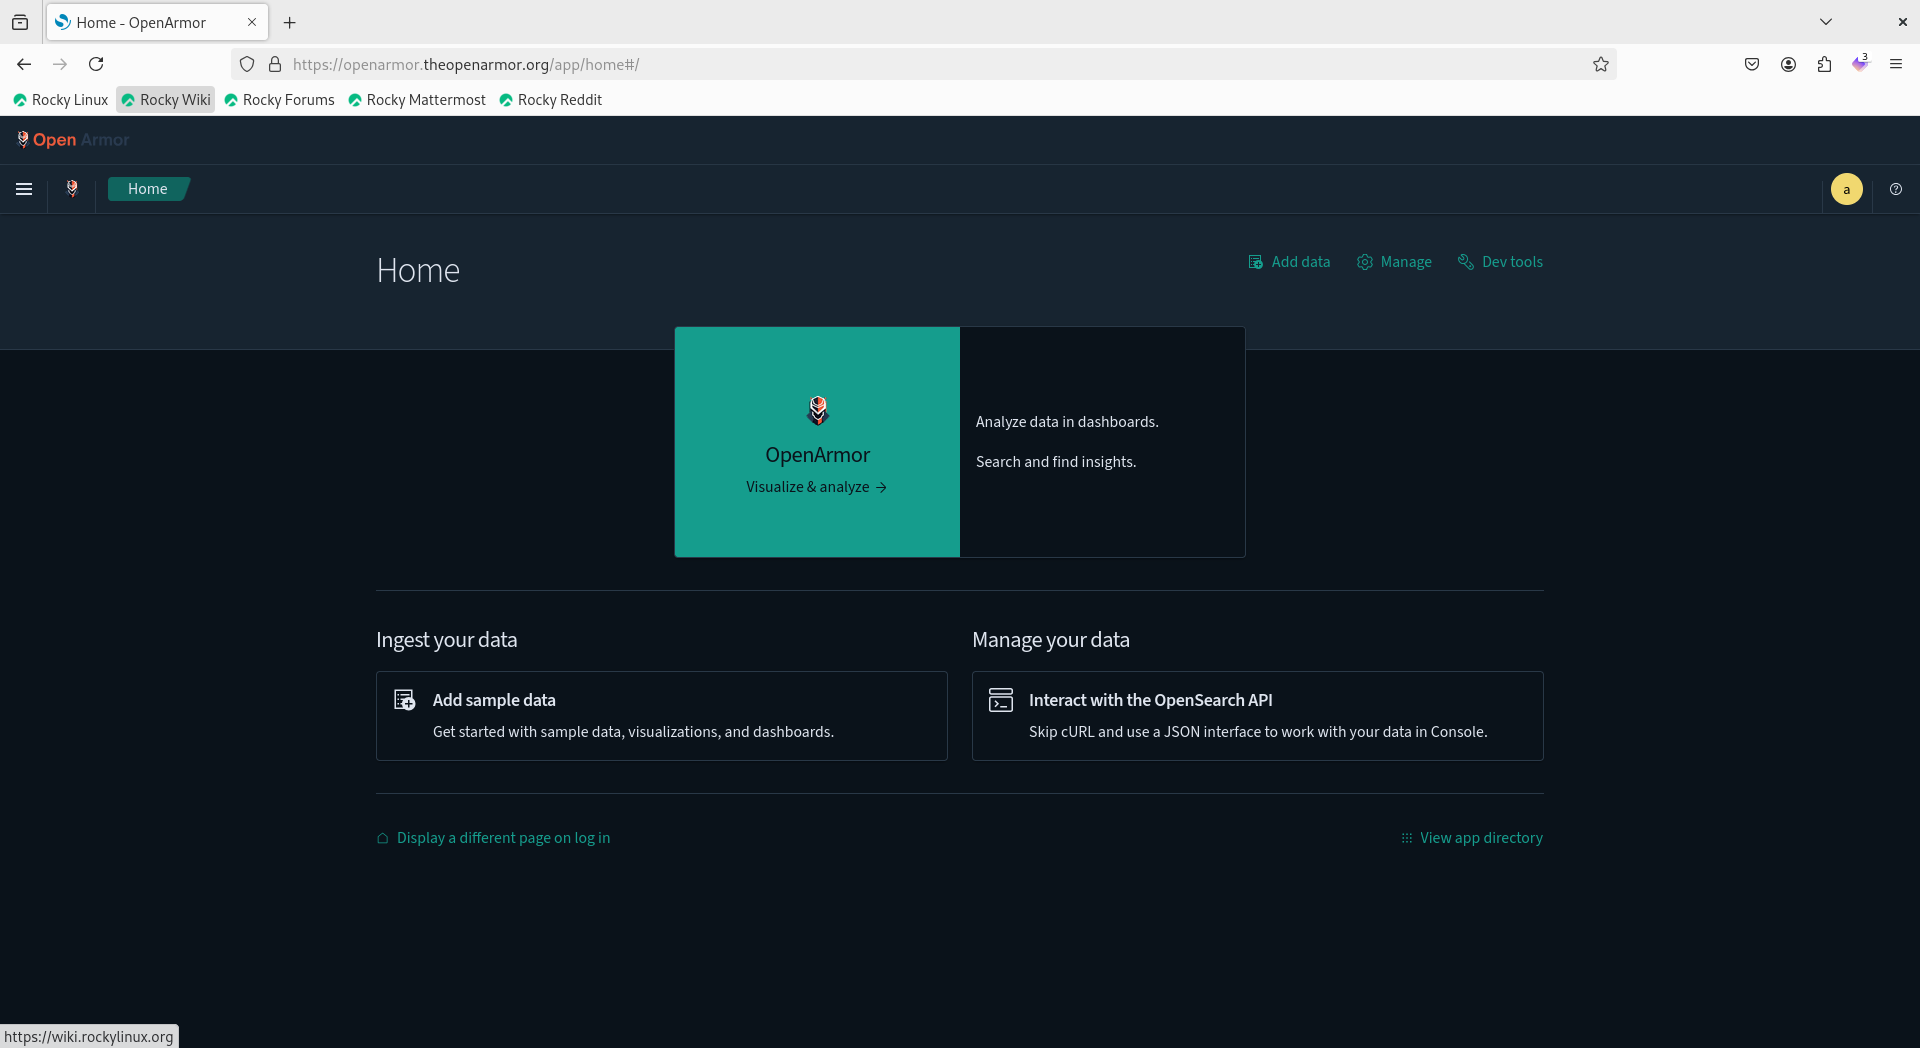
\includegraphics[width=0.7\textwidth]{openarmor-agent/2.png}
    \caption{Agent Setup Process}
    \label{fig:agent-setup}
\end{figure}

\subsection{Server Setup}
\begin{enumerate}
    \item Deploy OpenArmor server in a test environment.
    \item Configure server with test certificates and encryption keys.
    \item Set up test databases and indexers.
\end{enumerate}

\begin{figure}[h]
    \centering
    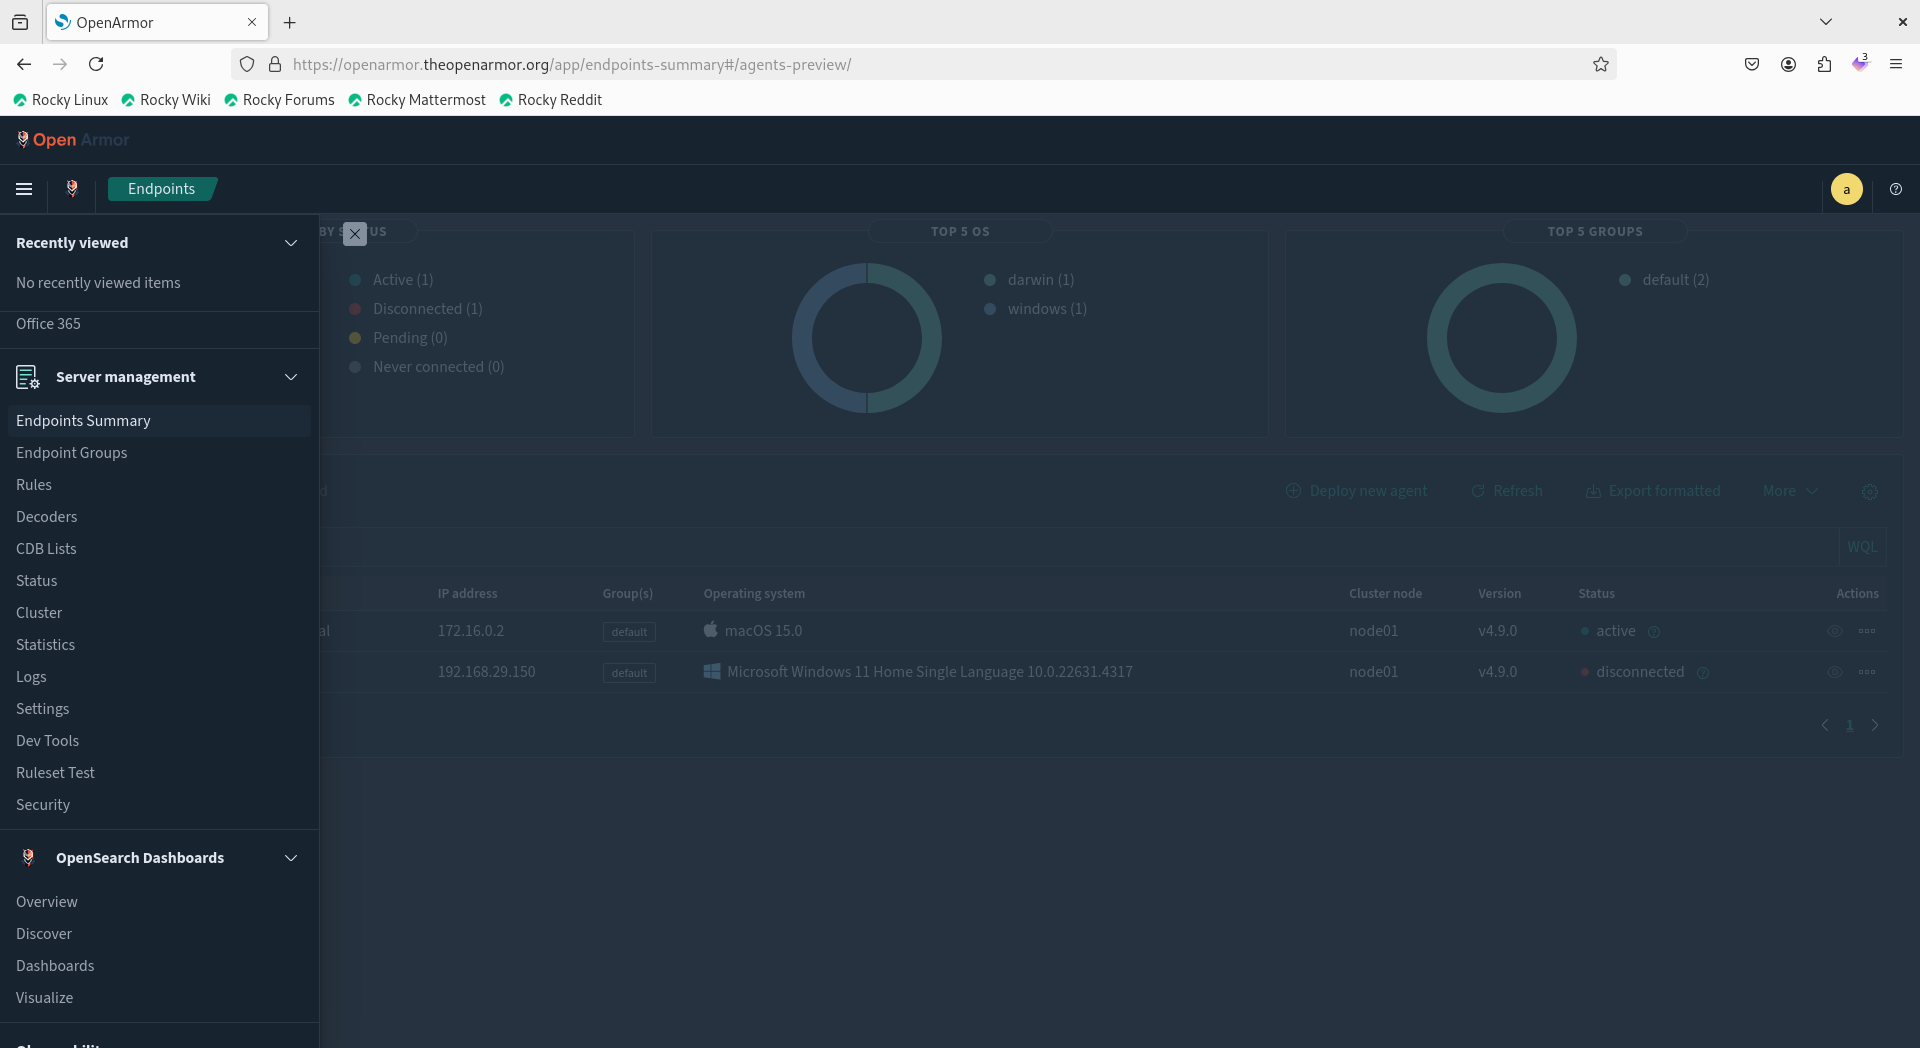
\includegraphics[width=0.7\textwidth]{openarmor-agent/3.png}
    \caption{Server Setup Configuration}
    \label{fig:server-setup}
\end{figure}

\subsection{Network Configuration}
\begin{enumerate}
    \item Configure firewalls to allow agent-server communication.
    \item Set up a test load balancer (if applicable).
    \item Prepare network monitoring tools for traffic analysis.
\end{enumerate}

\section{Functionality Testing}
\subsection{Agent Registration}
\begin{enumerate}
    \item Test new agent registration process.
    \item Verify agent appears in server's managed devices list.
    \item Check for proper agent ID assignment.
\end{enumerate}

\begin{figure}[h]
    \centering
    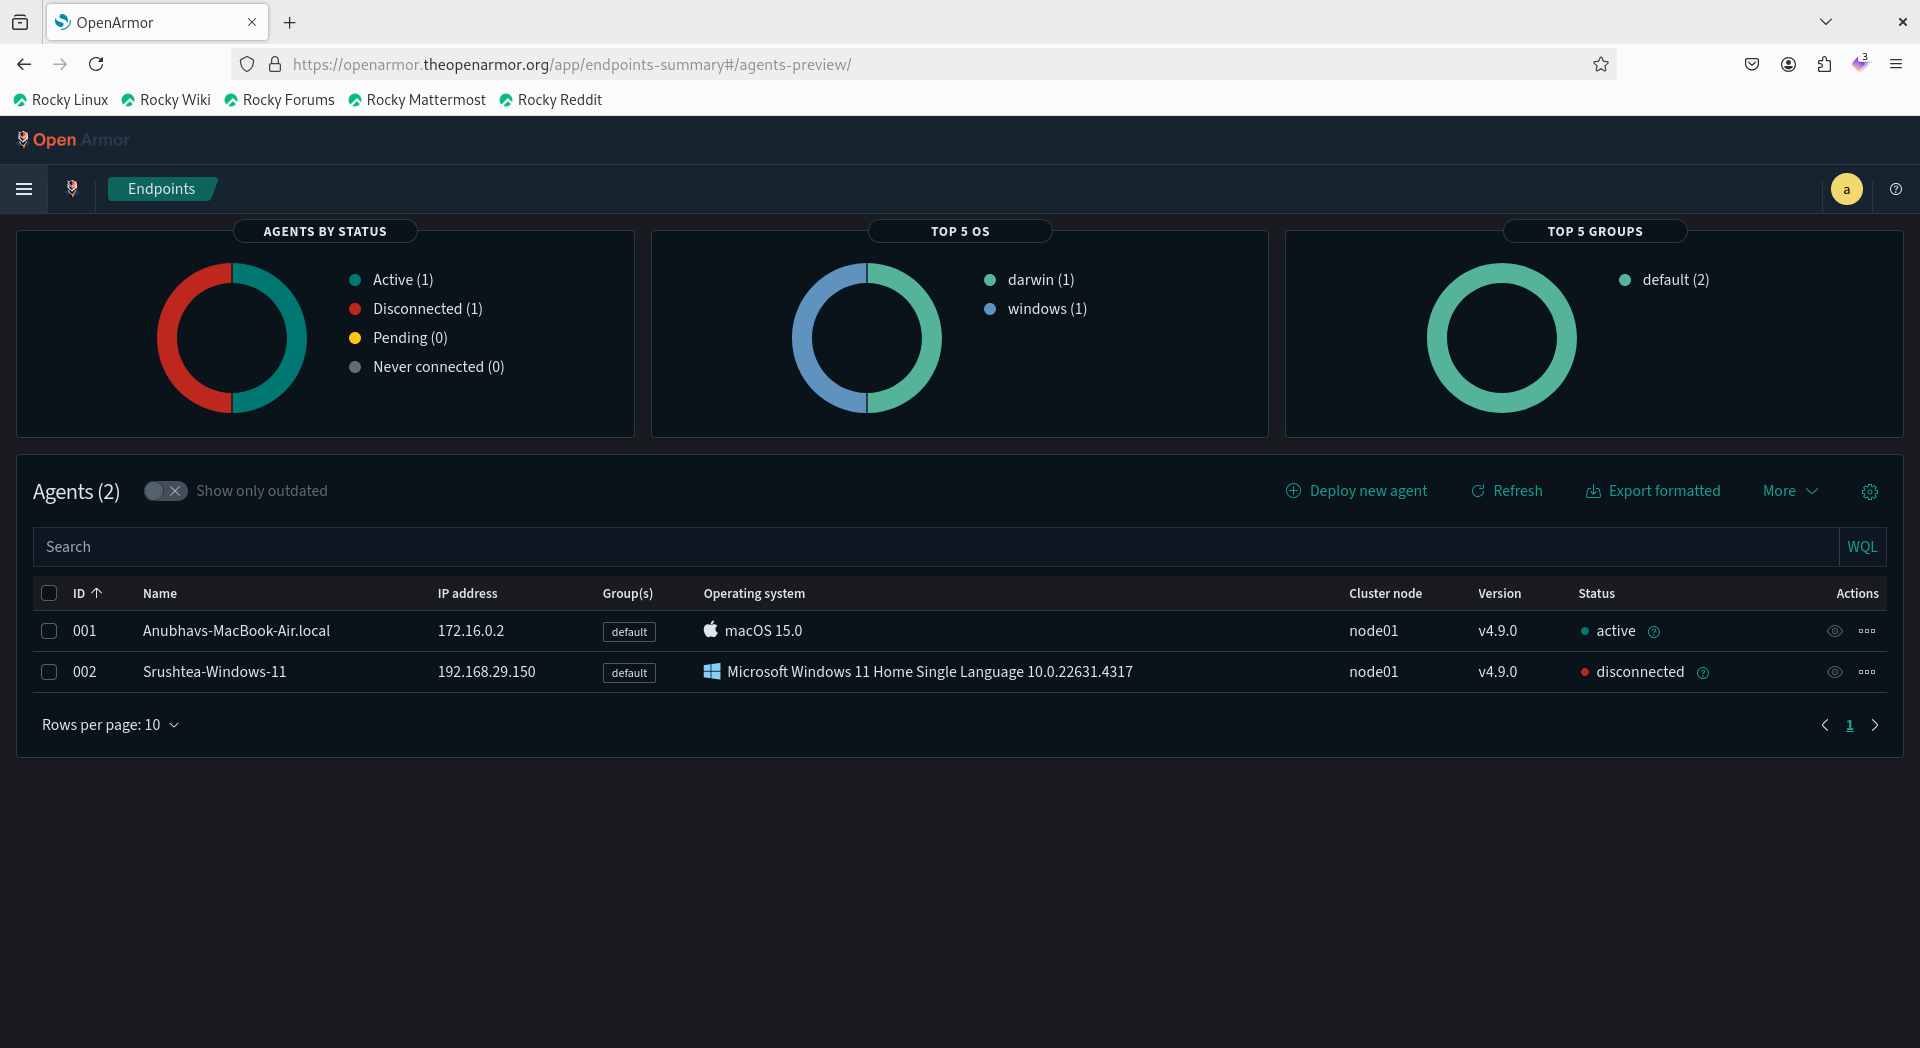
\includegraphics[width=0.8\textwidth]{openarmor-agent/4.png}
    \caption{Agent Registration Process}
    \label{fig:agent-registration}
\end{figure}

\subsection{Data Collection and Transmission}
\begin{enumerate}
    \item Trigger various events on the agent (file creation, network connection, etc.).
    \item Verify events are collected by the agent.
    \item Confirm events are successfully transmitted to the server.
    \item Check server logs for received data.
\end{enumerate}

\begin{figure}[h]
    \centering
    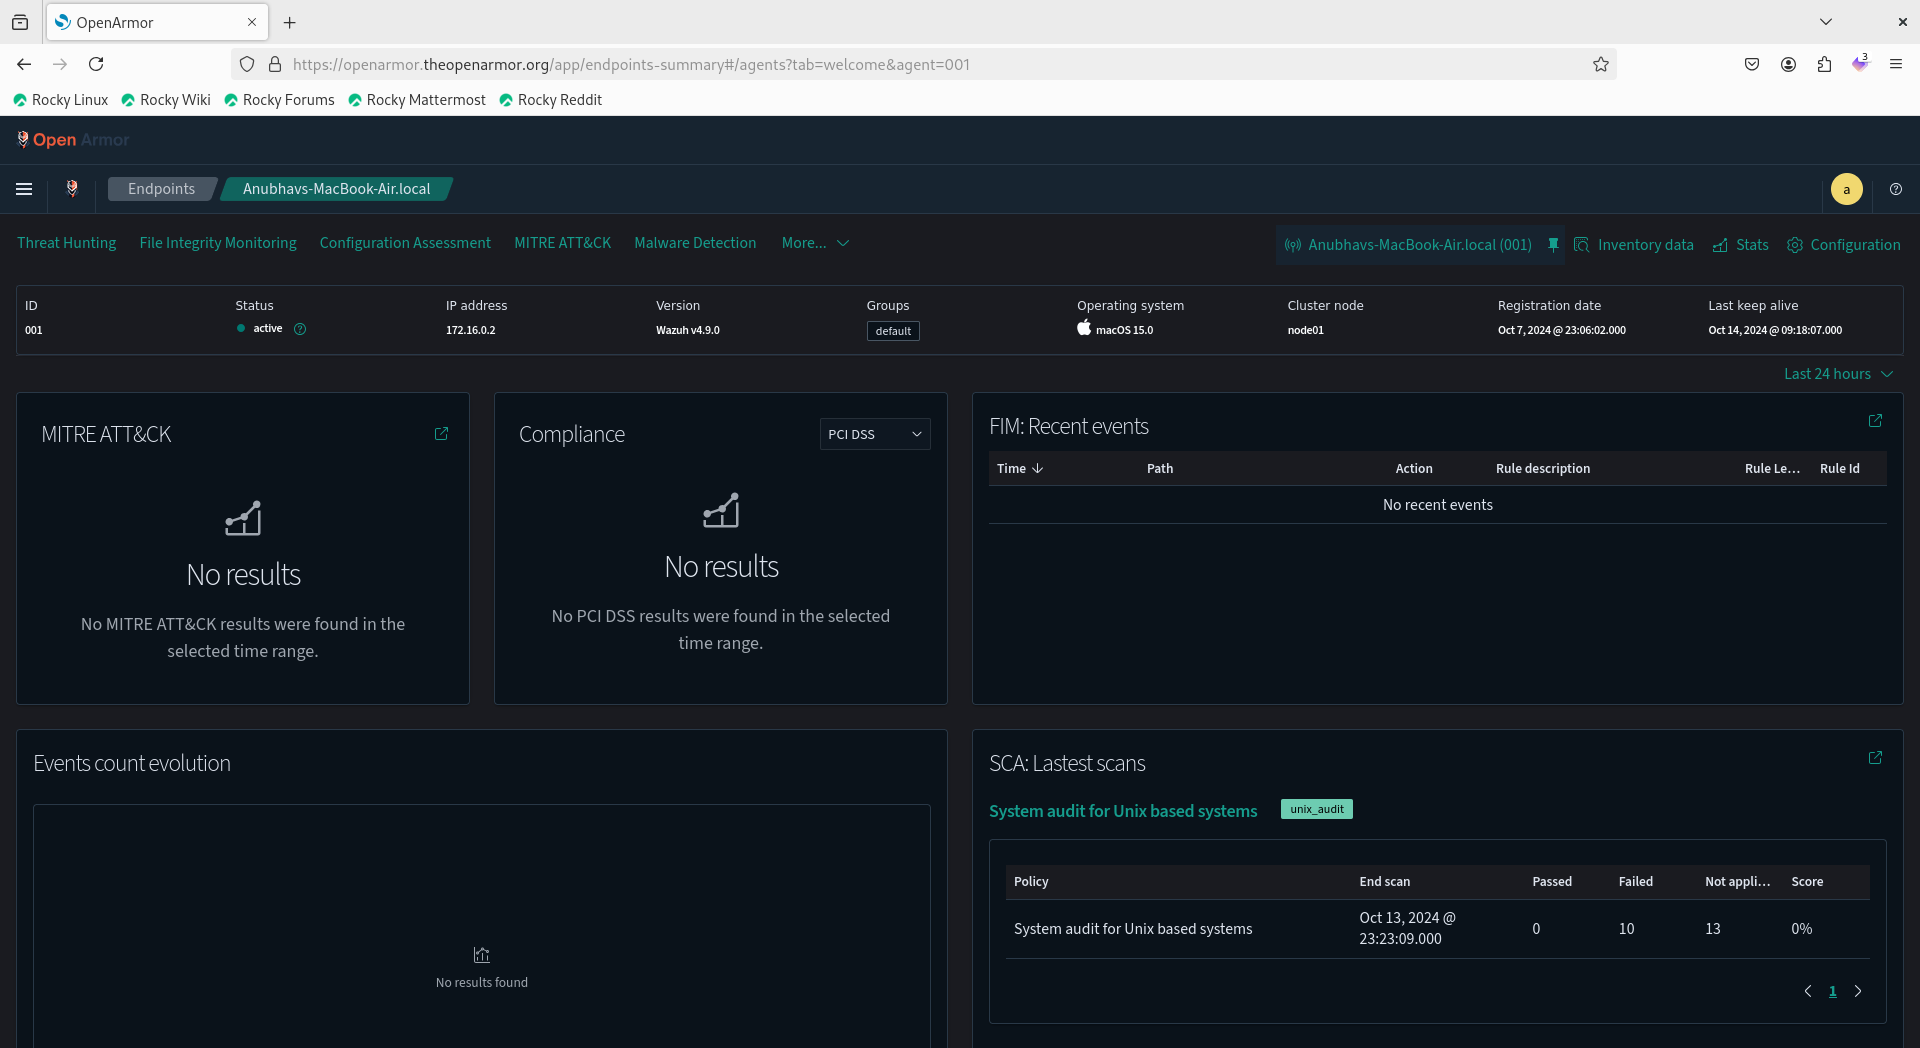
\includegraphics[width=0.7\textwidth]{openarmor-agent/5.png}
    \caption{Data Collection and Transmission Flow}
    \label{fig:data-collection}
\end{figure}

\subsection{Command and Control}
\begin{enumerate}
    \item Send configuration updates from server to agent.
    \item Issue commands (e.g., run query, update signatures) from server to agent.
    \item Verify agent acknowledges and executes commands.
    \item Check for command results reported back to the server.
\end{enumerate}

\section{Security Testing}
\subsection{Encryption}
\begin{enumerate}
    \item Capture network traffic between agent and server.
    \item Verify all traffic is encrypted (TLS inspection).
    \item Attempt to decrypt captured traffic with incorrect keys.
\end{enumerate}

\begin{figure}[h]
    \centering
    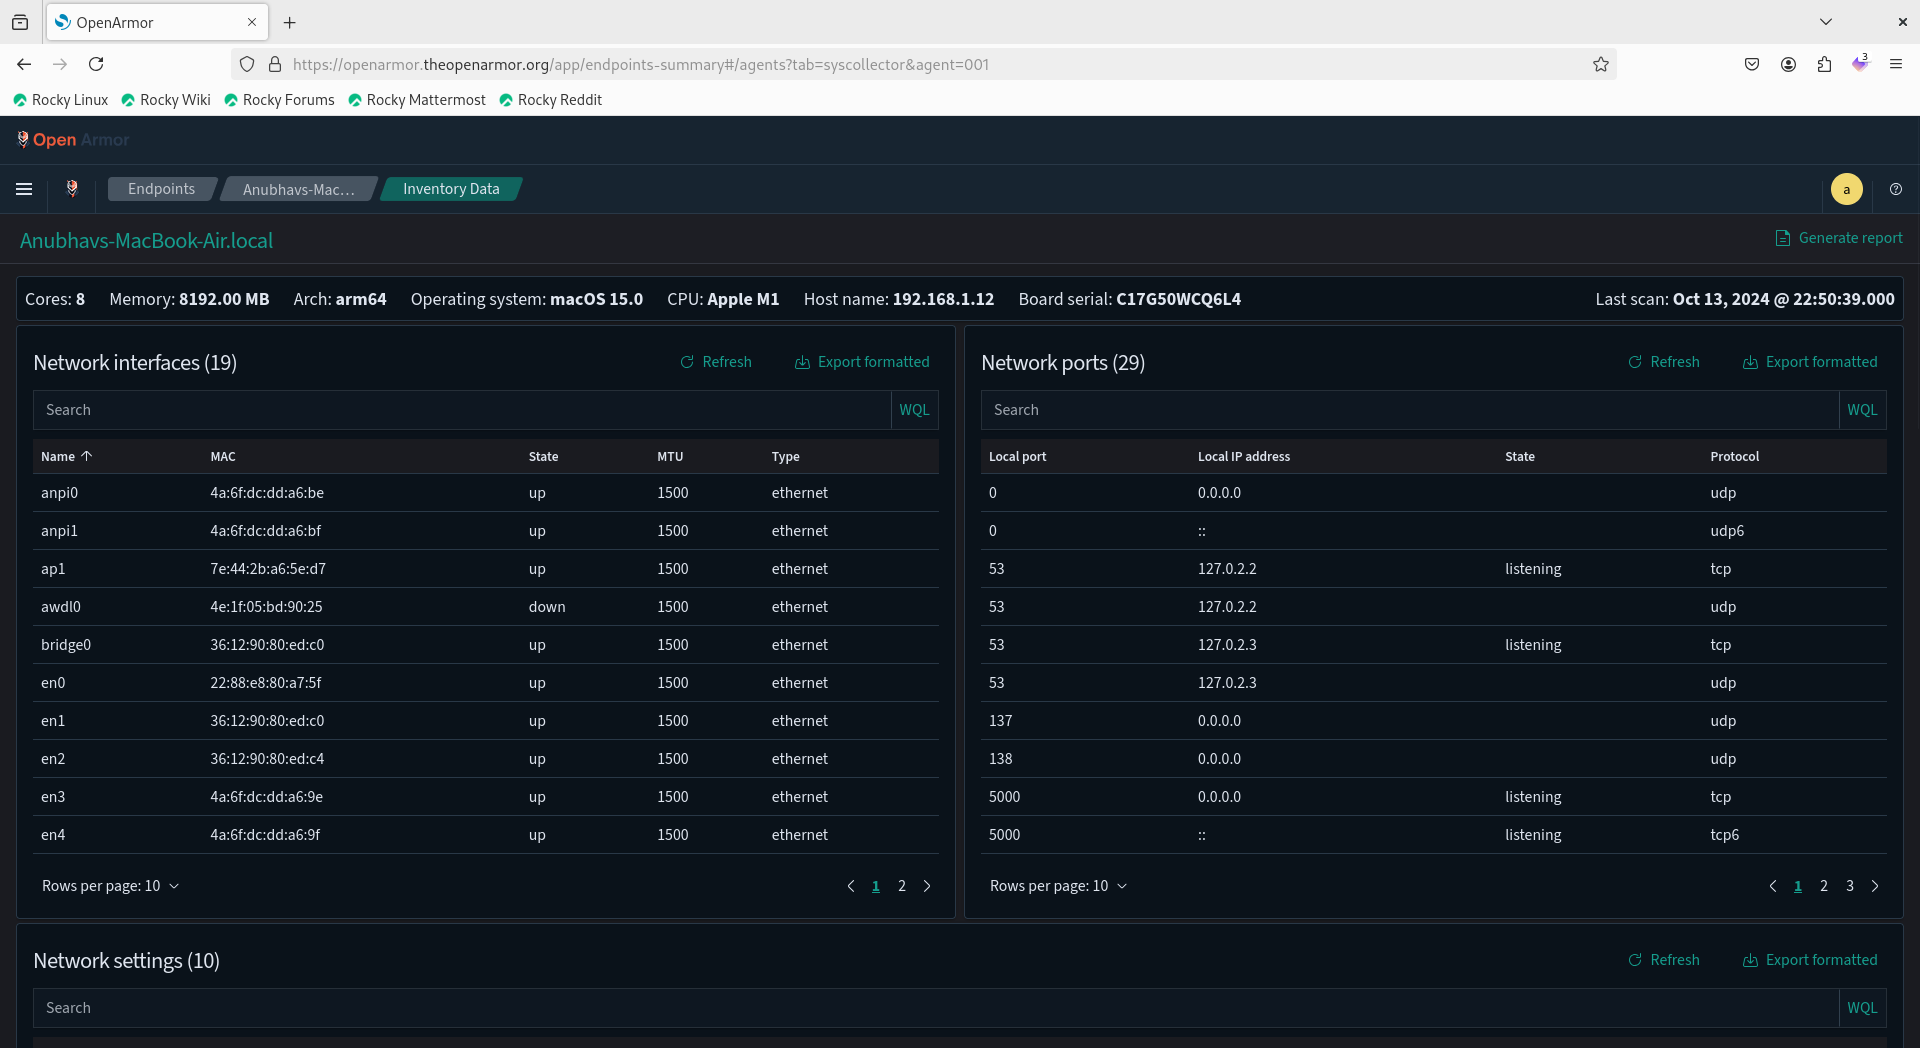
\includegraphics[width=0.8\textwidth]{openarmor-agent/6.png}
    \caption{Encryption Testing Procedure}
    \label{fig:encryption-testing}
\end{figure}

\subsection{Authentication}
\begin{enumerate}
    \item Attempt connection with invalid agent credentials.
    \item Test certificate-based authentication.
    \item Verify token-based session management.
\end{enumerate}

\subsection{Authorization}
\begin{enumerate}
    \item Test agent access to server resources with different permission levels.
    \item Attempt unauthorized command execution from agent to server.
    \item Verify data access controls on the server side.
\end{enumerate}

\section{Performance Testing}
\subsection{Load Testing}
\begin{enumerate}
    \item Simulate high event generation rate on agents.
    \item Monitor server performance under increased load.
    \item Test with multiple concurrent agent connections.
\end{enumerate}

\begin{figure}[h]
    \centering
    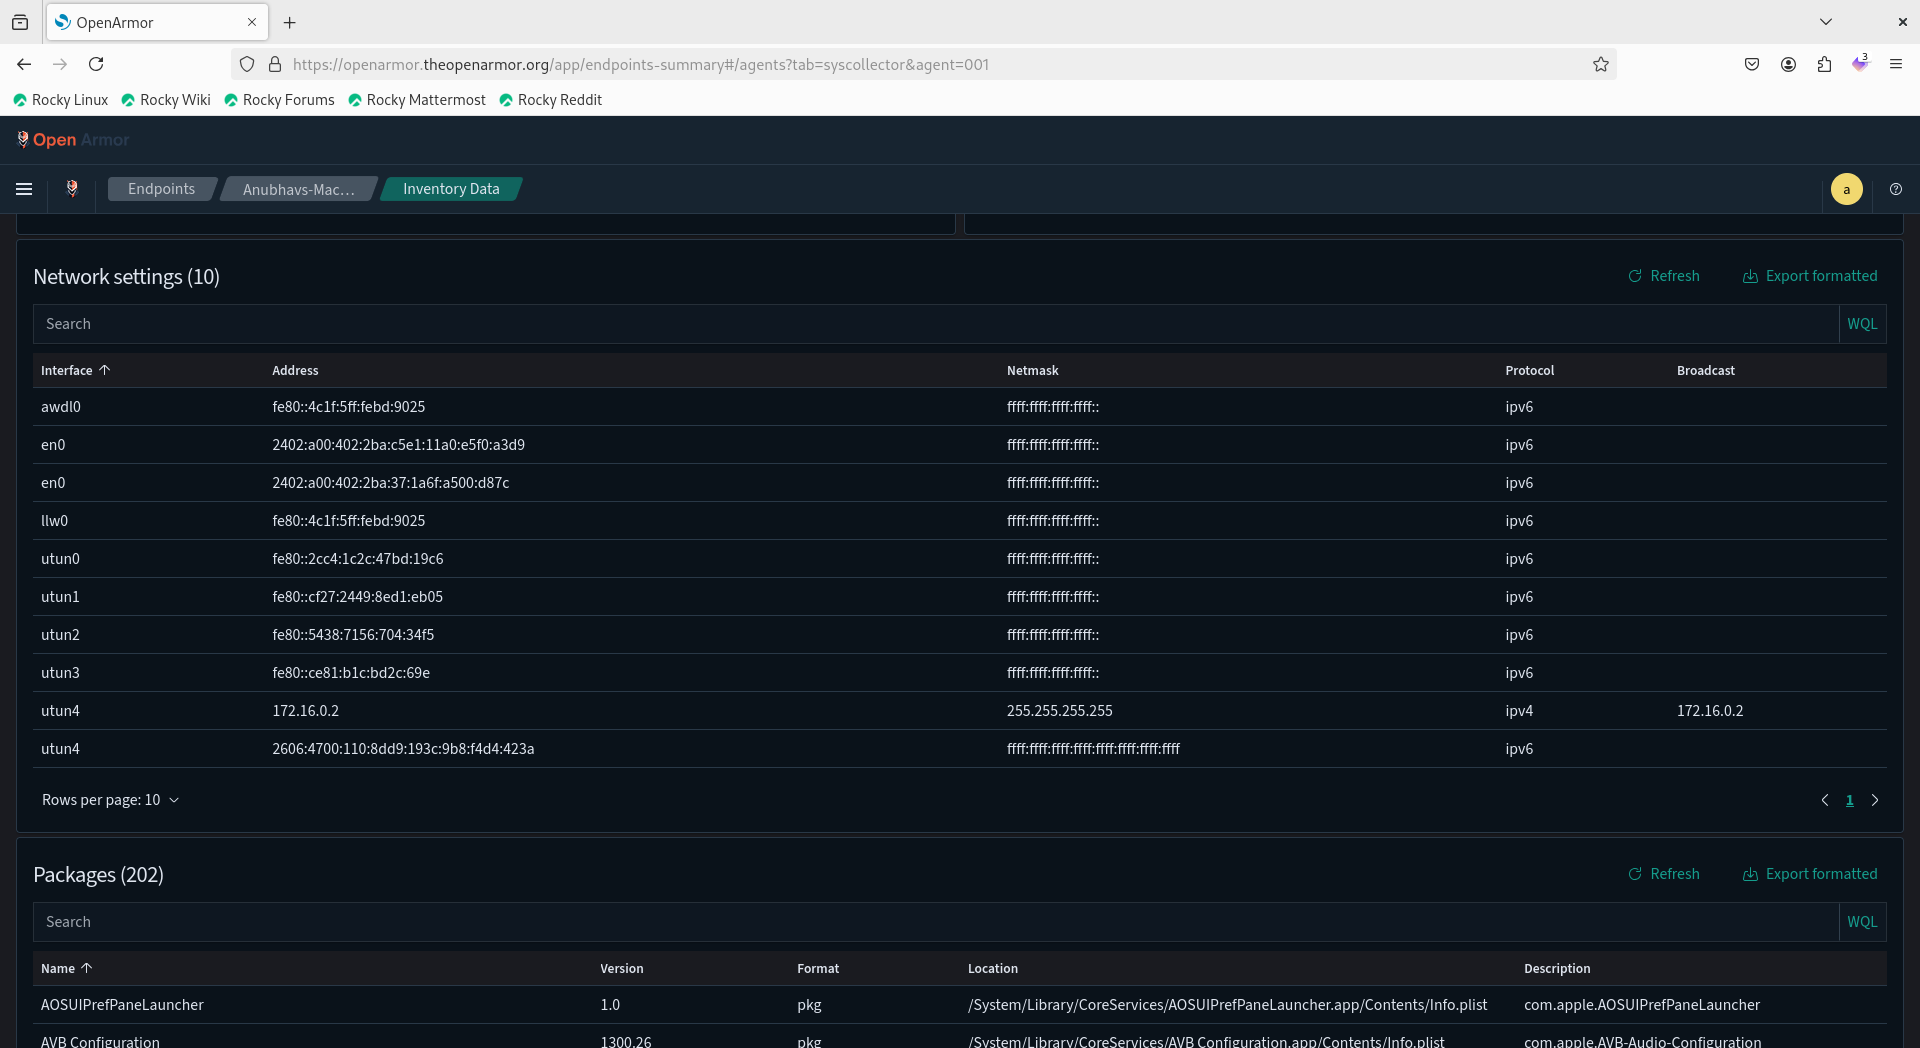
\includegraphics[width=0.7\textwidth]{openarmor-agent/7.png}
    \caption{Load Testing Scenario}
    \label{fig:load-testing}
\end{figure}

\subsection{Latency Testing}
\begin{enumerate}
    \item Measure round-trip time for agent-server communications.
    \item Test latency under various network conditions.
    \item Verify real-time alert capabilities.
\end{enumerate}

\subsection{Reliability Testing}
\begin{enumerate}
    \item Simulate network interruptions between agent and server.
    \item Test agent behavior during server unavailability.
    \item Verify data integrity and synchronization after reconnection.
\end{enumerate}

\section{Integration Testing}
\subsection{SIEM Integration}
\begin{enumerate}
    \item Verify agent data flow to SIEM system.
    \item Test SIEM alert generation based on agent data.
    \item Check SIEM dashboard for agent status and events.
\end{enumerate}

\begin{figure}[h]
    \centering
    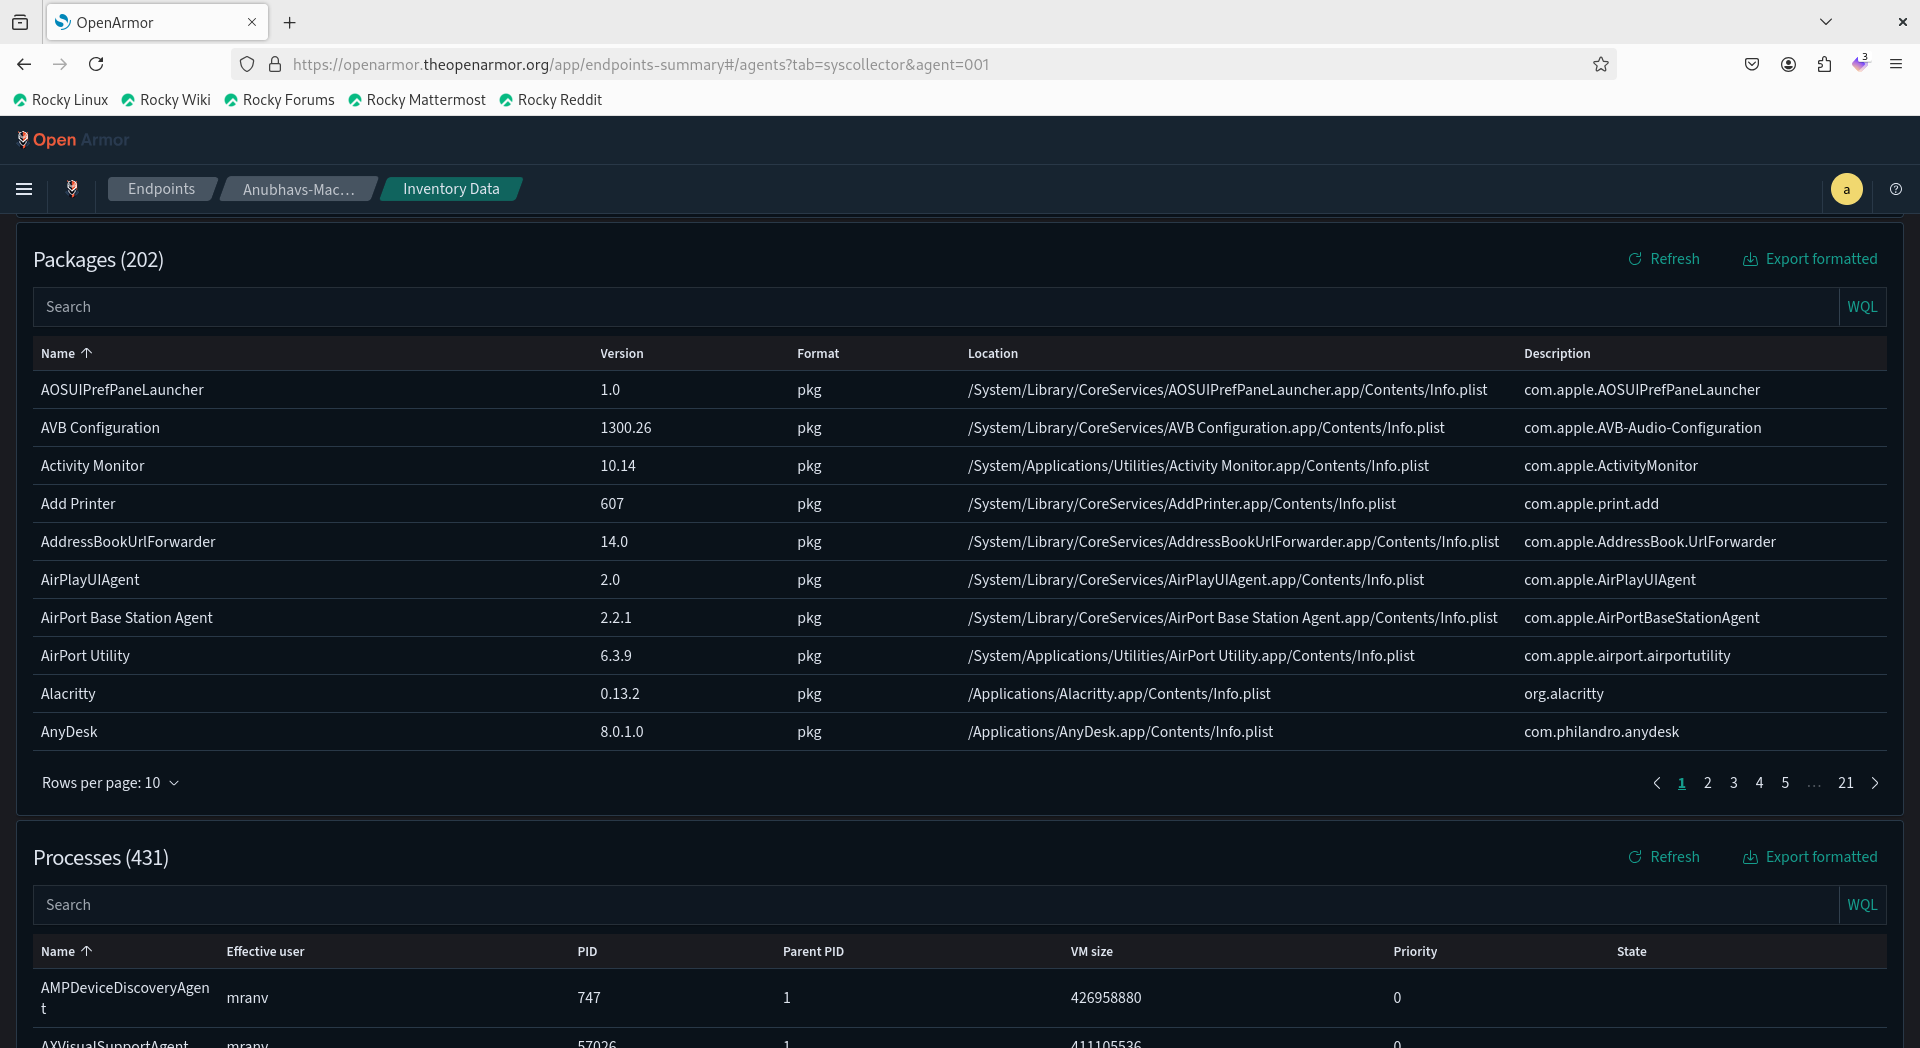
\includegraphics[width=0.8\textwidth]{openarmor-agent/8.png}
    \caption{SIEM Integration Architecture}
    \label{fig:siem-integration}
\end{figure}

\subsection{API Testing}
\begin{enumerate}
    \item Test RESTful API endpoints for agent management.
    \item Verify API authentication and rate limiting.
    \item Validate API responses for various agent operations.
\end{enumerate}

\section{User Acceptance Testing}
\subsection{Dashboard Functionality}
\begin{enumerate}
    \item Verify agent status display on OpenArmor dashboard.
    \item Test filtering and searching capabilities for agent data.
    \item Validate real-time updates of agent information.
\end{enumerate}

\subsection{Reporting}
\begin{enumerate}
    \item Generate reports on agent status and events.
    \item Verify accuracy of agent data in reports.
    \item Test scheduled and on-demand report generation.
\end{enumerate}

\begin{figure}[h]
    \centering
    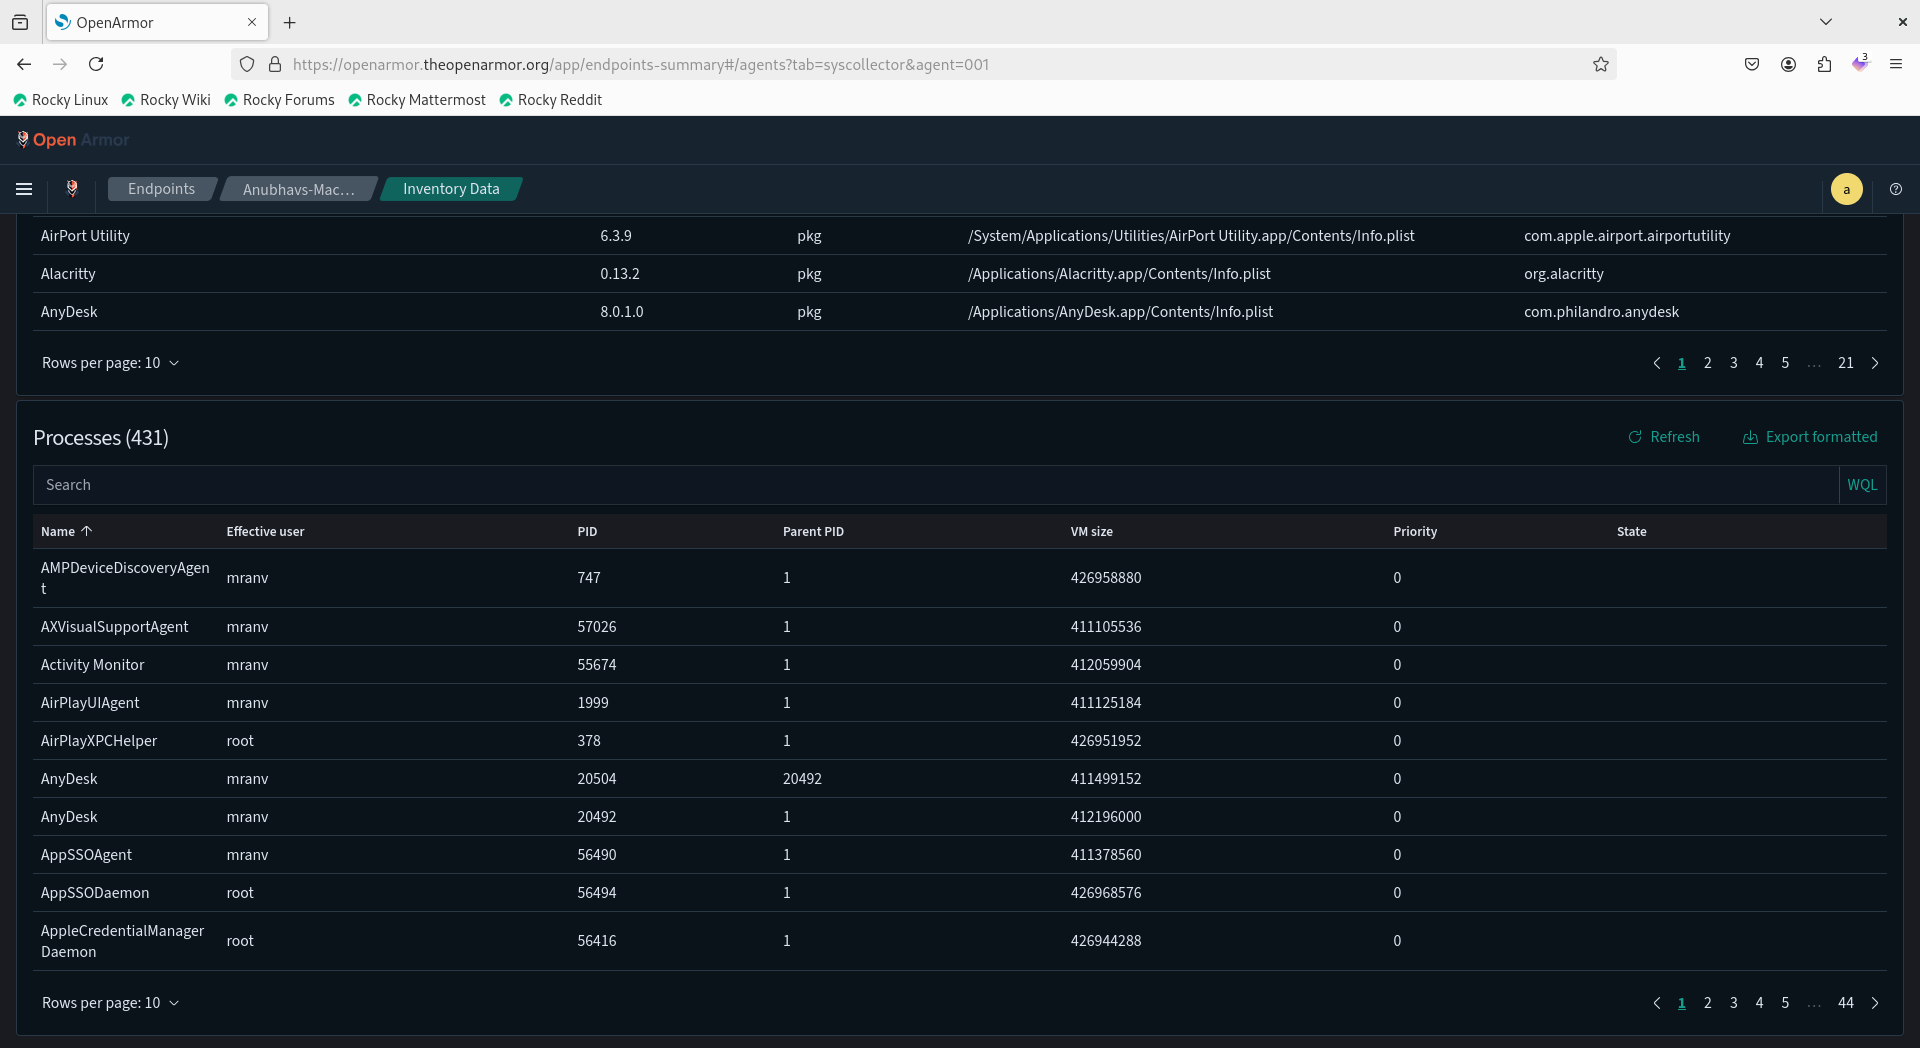
\includegraphics[width=0.7\textwidth]{openarmor-agent/9.png}
    \caption{Sample OpenArmor Dashboard and Reporting Interface}
    \label{fig:dashboard-reporting}
\end{figure}

\section{Conclusion}
This testing documentation provides a comprehensive guide for verifying the OpenArmor agent-server communication. By following these procedures and utilizing the illustrated test scenarios, testers can ensure the reliability, security, and performance of the OpenArmor system. Regular execution of these tests will help maintain the integrity of the agent-server interaction as the system evolves.